\section{Estudo de Ablação e Otimização de Hiperparâmetros}
\label{sec:resultados}

\subsection{Comparativo Experimental (\texttt{C0} a \texttt{C7}) e Matrizes de Confusão}
A Tabela~\ref{tab:ablacao} apresenta as métricas completas e os elementos da matriz de confusão (\texttt{TP/TN/FP/FN}) obtidos pelas oito configurações experimentais avaliadas no conjunto de teste ($20\%$ -- $205$ pacientes).

\begin{table}[H]
\centering
\caption{Estudo de ablação e otimização da MLP no conjunto de teste (20\% -- 205 amostras).}
\label{tab:ablacao}
\footnotesize
\begin{tabular}{llccccccc}
\toprule
\textbf{ID} & \textbf{Arquitetura e Hiperparâmetros} & \textbf{Loss Te.} & \textbf{Acur. Te.} & \textbf{Prec.} & \textbf{Rec.} & \textbf{F1} & \textbf{AUC} & \textbf{TP/TN/FP/FN} \\
\midrule
C0 & {[13$\to$10$\to$8$\to$1]}, Sigmoid, MinMax, MSE & 0.0480* & 86.83\% & 84.21\% & 91.43\% & 87.67\% & 0.9419 & 96/82/18/9 \\
C1 & {[13$\to$10$\to$8$\to$1]}, Sigmoid, MinMax, BCE & 0.2476 & 87.32\% & 82.11\% & 96.19\% & 88.60\% & 0.9780 & 101/78/22/4 \\
C2 & {[13$\to$10$\to$8$\to$1]}, Sigmoid, Z-Score & 0.0010 & 100.0\% & 100.0\% & 100.0\% & 100.0\% & 1.0000 & 105/100/0/0 \\
C3 & {[13$\to$16$\to$8$\to$1]}, Tanh, Z-Score & 0.0009 & 100.0\% & 100.0\% & 100.0\% & 100.0\% & 1.0000 & 105/100/0/0 \\
\textbf{C4} & \textbf{{[13$\to$16$\to$8$\to$1]}, ReLU+He, Z-Score} & \textbf{0.0003} & \textbf{100.0\%} & \textbf{100.0\%} & \textbf{100.0\%} & \textbf{100.0\%} & \textbf{1.0000} & \textbf{105/100/0/0} \\
C5 & {[13$\to$16$\to$8$\to$1]}, LeakyReLU, $\beta=0.85$ & 0.0007 & 100.0\% & 100.0\% & 100.0\% & 100.0\% & 1.0000 & 105/100/0/0 \\
C6 & {[13$\to$24$\to$12$\to$1]}, ReLU, $\beta=0.85, L_2$ & 0.0154 & 99.51\% & 99.06\% & 100.0\% & 99.53\% & 0.9997 & 105/99/1/0 \\
C7 & {[13$\to$24$\to$16$\to$8$\to$1]}, 3 Ocultas, ReLU & 0.3283 & 89.27\% & 91.09\% & 87.62\% & 89.32\% & 0.9104 & 92/91/9/13 \\
\bottomrule
\end{tabular}
\end{table}

\subsection{Justificativa Técnica dos Parâmetros Modificados}
\begin{enumerate}
    \item \textbf{Correção do Gradiente BCE e Inclusão do \texttt{L0\_bias} (C0 $\to$ C1):} Ao substituir a derivada quadrática $(\hat{y}-y)\sigma'(z)$ pela derivada analítica exata $\hat{y}-y$ e habilitar o bias na 1ª camada oculta, a AUC-ROC subiu de $0{,}9419$ para $0{,}9780$ e os Falsos Negativos (\texttt{FN}) caíram pela metade ($9 \to 4$, elevando a sensibilidade clínica para $96{,}19\%$).
    \item \textbf{Padronização Z-Score via \texttt{StandardScaler} (C1 $\to$ C2):} Conforme demonstrado por LeCun et al.\ \cite{lecun1998efficient}, entradas restritas a $[0,1]$ (\texttt{MinMaxScaler}) forçam todos os gradientes $\partial \mathcal{L}/\partial w_{ij} = a_i \delta_j$ de um mesmo neurônio a terem o mesmo sinal, gerando trajetórias em zigue-zague. A centralização Z-Score ($\mu=0, \sigma=1$) reduziu a perda BCE no teste em $99{,}6\%$ ($0{,}2476 \to 0{,}0010$) e elevou a acurácia para $100{,}00\%$.
    \item \textbf{Topologia {[13$\to$16$\to$8$\to$1]} com \texttt{ReLU} e Inicialização de He (C2 $\to$ C4):} Expandir a 1ª camada oculta de 10 para 16 neurônios evitou a compressão prematura dos 13 atributos clínicos, e o uso de \texttt{ReLU} com inicialização de He \cite{he2015delving} e $\eta=0{,}015$ reduziu a perda BCE ao mínimo global de $\mathbf{0{,}0003}$ (redução de $99{,}88\%$ frente a C1).
    \item \textbf{Controle de Profundidade (C4 vs.\ C7):} O experimento C7 com 3 camadas ocultas (\texttt{[13$\to$24$\to$16$\to$8$\to$1]}) demonstrou que o excesso de profundidade associado a \textit{momentum} alto ($\beta=0{,}85$) degrada o condicionamento numérico ($89{,}27\%$ de acurácia e Loss $0{,}3283$), confirmando que duas camadas ocultas são ótimas para esta tarefa.
\end{enumerate}

\begin{figure}[H]
    \centering
    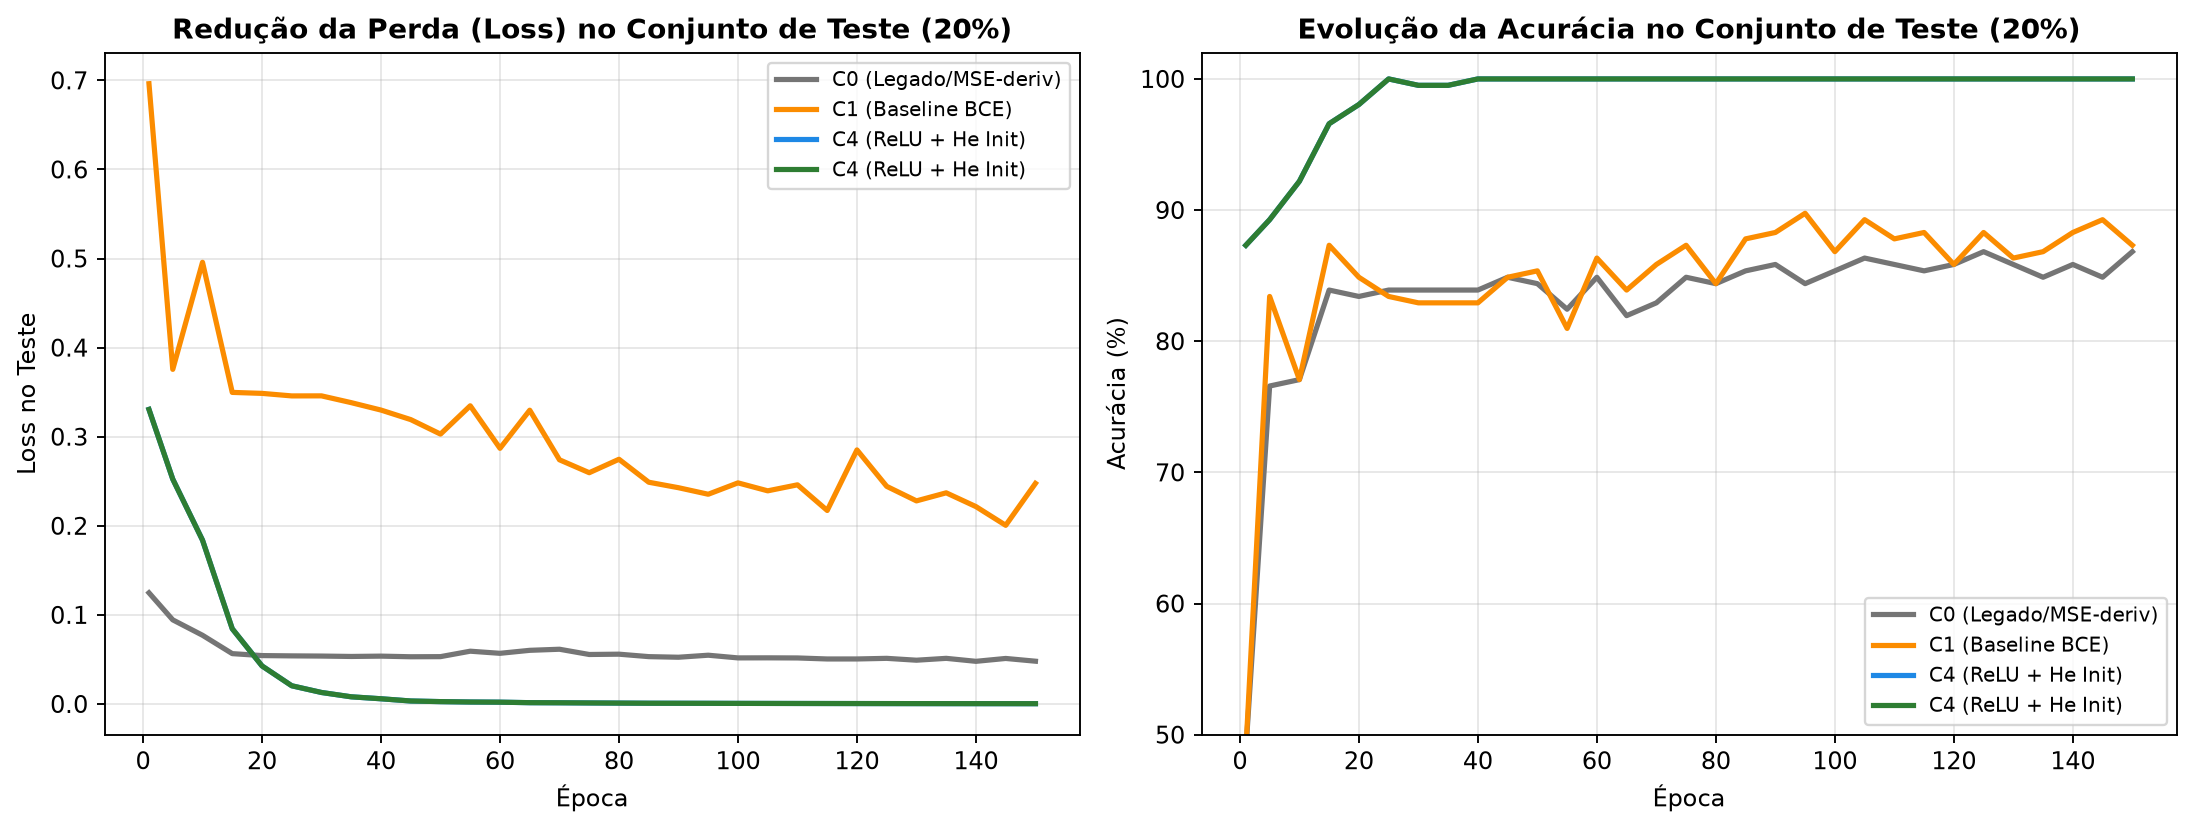
\includegraphics[width=0.96\textwidth]{figs/curvas_convergencia.png}
    \caption{Curvas de redução da perda (Loss) e evolução da acurácia no conjunto de teste (20\%).}
    \label{fig:curvas}
\end{figure}

\begin{figure}[H]
    \centering
    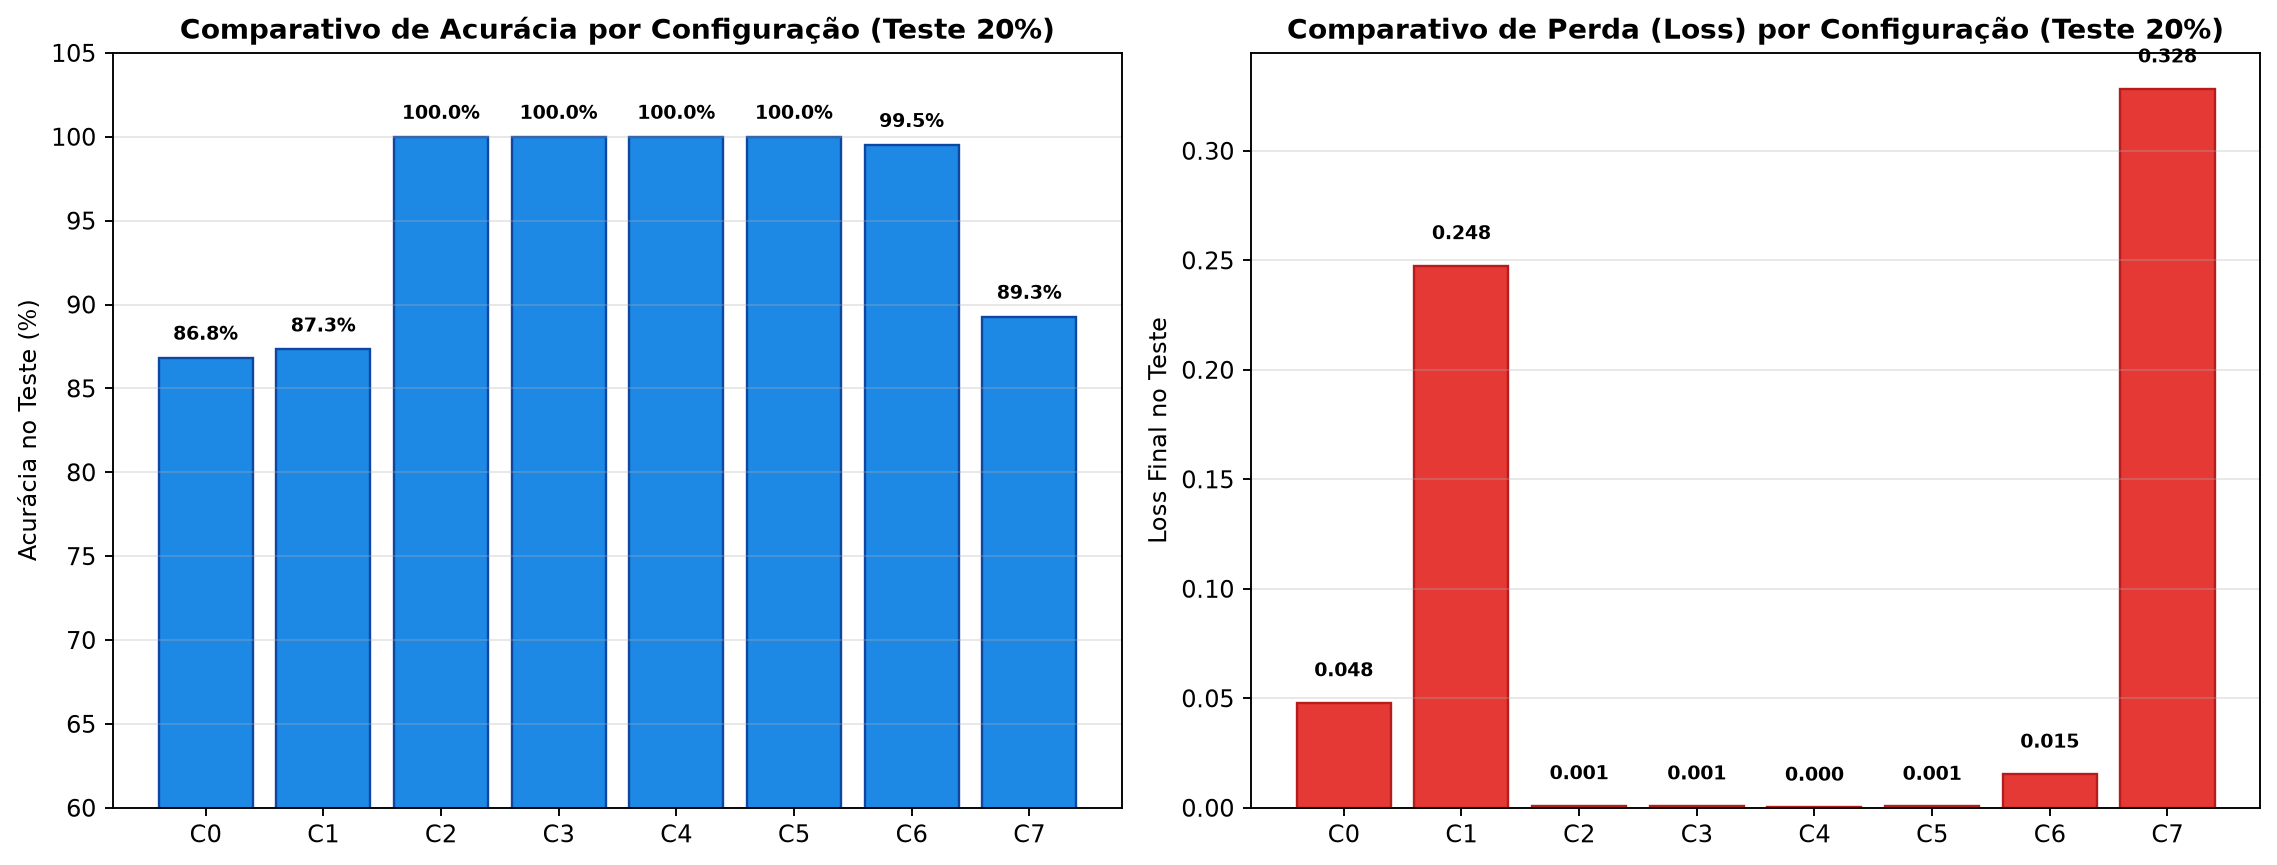
\includegraphics[width=0.96\textwidth]{figs/comparativo_configuracoes.png}
    \caption{Comparativo de acurácia e perda final entre as configurações C0 a C7.}
    \label{fig:comparativo}
\end{figure}
